\documentclass{article}

\usepackage{circuitikz}
\usepackage[T1]{fontenc} 
\usepackage[UTF8]{inputenc}
\usepackage{amsmath}
\usepackage{amssymb}
\usepackage{fancyhdr}
\usepackage{graphicx}
\usepackage{hyperref}
\usepackage{tikz}
  \usetikzlibrary{arrows}
  \usetikzlibrary{shapes}
  \usetikzlibrary{arrows.meta,topaths}
  \usetikzlibrary{bending}
  \usetikzlibrary{calc}
\usepackage{anyfontsize}
\usepackage{sectsty}
\usepackage{../assets/scripts/tex/color-env}
\usepackage{anyfontsize}
\usepackage{xcolor}
\definecolor{DarkGreenBlue}{HTML}{264653}
\definecolor{LightGreenBlue}{HTML}{2A9D8F}
\definecolor{LightOrange}{HTML}{E9C46A}
\definecolor{DarkOrange}{HTML}{F4A261}
\definecolor{RedOrange}{HTML}{E76F51}
\definecolor{BrightRed}{HTML}{D62828}
\definecolor{DeepBlue}{HTML}{003049}



\usepackage[ngerman]{babel}
\title{Elektrotechnik 1 - Praktikum 3}


\usepackage[
  includehead,
  headheight = 17mm,
  footskip = \dimexpr\headsep+\ht\strutbox\relax,
  tmargin = 0mm,
  bmargin = \dimexpr17mm+2\ht\strutbox\relax,
]{geometry}





\pagestyle{fancy}
\fancyhead[L]{\leftmark}
\fancyhead[R]{}
\fancyfoot[L]{}
\fancyfoot[C]{\thepage}
\fancyfoot[R]{
\includegraphics[scale=0.2]{../assets/images/haw.jpg}}
\renewcommand\headrulewidth{0.5pt}

\begin{document}

\thispagestyle{empty}
\begin{tikzpicture}[remember picture,overlay]

  \fill[DeepBlue] (current page.south west) rectangle (current page.north east);

  \begin{scope}

    \foreach \i in {2.5,...,22}
      {
        \node[rounded corners, DeepBlue!90,draw ,regular polygon, regular polygon sides=6, minimum size=\i cm, ultra thick] at ($(current page.west)+(2.5,-5)$) {} ;
      }

  \end{scope}

  \node[rounded corners,fill=DeepBlue!95,text =DeepBlue!5,regular polygon,regular polygon sides=6, minimum size=2.5 cm,inner sep=0,ultra thick] at ($(current page.west)+(2.5,-5)$) {\LARGE \bfseries 2020};

  \foreach \i in {0.5,...,22}
    {
      \node[rounded corners,DeepBlue!90,draw,regular polygon,regular polygon sides=6, minimum size=\i cm,ultra thick] at ($(current page.north west)+(2.5,0)$) {} ;
    }

  \foreach \i in {0.5,...,22}
    {
      \node[rounded corners,DeepBlue!98,draw,regular polygon,regular polygon sides=6, minimum size=\i cm,ultra thick] at ($(current page.north east)+(0,-9.5)$) {} ;
    }

  \foreach \i in {12}
    {
      \node[fill = DeepBlue,rounded corners,draw=DeepBlue,regular polygon,regular polygon sides=6, minimum size=\i cm,ultra thick] at ($(current page.south east)+(-0.2,-0.45)$) {} ;
    }


  \foreach \i in {21,...,6}
    {
      \node[DeepBlue!95,rounded corners,draw,regular polygon,regular polygon sides=6, minimum size=\i cm,ultra thick] at ($(current page.south east)+(-0.2,-0.45)$) {} ;
    }

  \node[left,DeepBlue!5,minimum width=0.625*\paperwidth,minimum height=3cm, rounded corners] at ($(current page.north east)+(0,-9.5)$){{\fontsize{25}{30} \selectfont \bfseries ET2 - Praktikum 6}};

  \node[left,DeepBlue!10,minimum width=0.625*\paperwidth,minimum height=2cm, rounded corners] at ($(current page.north east)+(0,-11)$){{\huge \textit{Transiente Vorgänge}}};

  \node[left,DeepBlue!5,minimum width=0.625*\paperwidth,minimum height=2cm, rounded corners] at ($(current page.north east)+(0,-13)$){{\Large \textsc{Florian Tietjen\hspace{0.5cm}Eric Antosch}}};

\end{tikzpicture}

\newpage
\thispagestyle{empty}

\tableofcontents


\newpage

\section{Vorbereitung}
Im fünften Praktikum werden die fortgeschrittenen Funktionen und Anwendungsmöglichkeiten eines Oszilloskops, insbesondere das Messen einmaliger ablaufender Schaltvorgänge.
Dafür wird die Cursor-Messfunktion und die Triggerart SINGLE SEQUENCE verwendet.
Zudem wird der Einfluss eines Tastteilers untersucht.
 
\subsection{Funktion eines Tastteilers}
Ein Tastteiler, auch Prüfling oder Tastkopf genannt, ist ein Messmittel, welches am Oszilloskop angeschlossen wird. Dabei handelt es sich um ein Koaxialkabel, welches das Oszilloskop elektrisch sowie physisch mit der Signalquelle verbindet.
 
\subsection{Funktion und Aufbau eines Relais}
Ein Relais ist vereinfacht gesagt ein elektromagnetischer Schalter, welcher durch Anlegen einer Spannung seine Ein- und Ausgänge schließt oder öffnet.
 
\subsection{Funktion einer Freilaufdiode}
Freilaufdioden sind Dioden, die zum Schutz vor Überspannung beim Abschalten einer induktiven Last dienen.
Nach dem Abschalten der Versorgungsspannung sorgt die Selbstinduktion einer Spule dafür, dass der Strom zunächst in der ursprünglichen Richtung weiter fließt. 
Ohne Freilaufdiode führt das zu einer Spannungsspitze, die sich zur Betriebsspannung addiert und dabei elektrische Bauteile beschädigen könnte.
Mit einer Freilaufdiode wird die Spannungsspitze jedoch auf die Durchlassspannung der Diode (bei Siliziumdioden etwa 0,7 V) begrenzt. 
\newpage

\section{Zeitmessung}

\begin{task}
    TIn dieser Aufgabe wollen wir den genauen Verlauf eines Rechtecksignals aus einem Funktionsgenerator analysieren.
\end{task}
\begin{devlist}
    T\begin{itemize}
        \item Oszilloskop
        \item Funktionsgenerator
    \end{itemize}
\end{devlist}
Wir wollen nun zunächst die Anstiegs - und Abfallzeit bestimmen. Dazu messen wir die Zeit, die der Impuls benötigt, um von 10\%
vom absoluten Spannungsbodens bis zu 10\% vom absoluten Spannungsdach zu kommen. Diese Zeit nennen wir Anstiegszeit $t_{rise}= $ . Gleichermaßen
messen wir die Zeit von 10\% vom absoluten Spannungsdach bis zu 10\% vom absoluten Spannungsboden. Diese Zeit nennen wir Abfallzeit $t_{fall} = $.

Mithilfe des Oszilloskops bestimmen wir nun die Frequenz $\mathrm{f} = $ und das Tastverhältnis $\mathrm{a} = \frac{t_{high}}{T} = $.

\newpage


\section{Einschalt- und Ausschaltvorgang an einem Relais}

\begin{task}
    TIn dieser Aufgabe wollen wir die Funktionsweise, sowie die entstehenden Spannungen und Ströme bei Schaltvorgängen mit Relais
    genauer analysieren. Dazu verwenden wir eine einfache Schaltung, die sich in Steuer- und Laststromkreis aufteilt. Der Shunt-Widerstand $R_M = 100\Omega$ dient als Messmittel
    zum Bestimmen der Ströme.
\end{task}
\begin{figure}[h]
    \begin{center}
        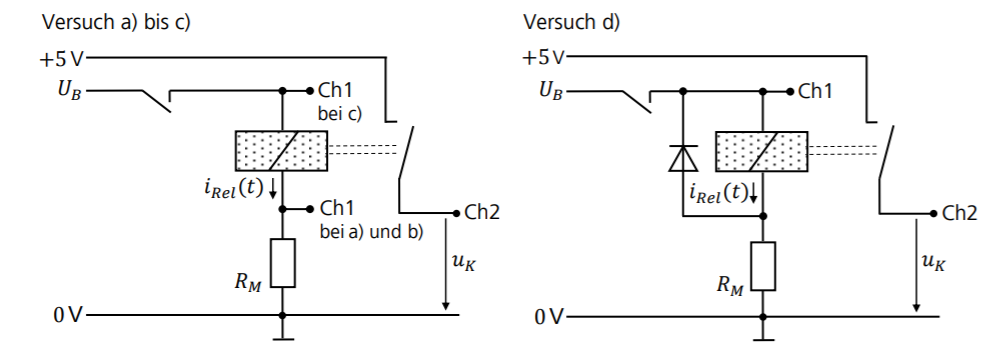
\includegraphics[scale=0.8]{../assets/images/ET2P4/Schaltplan2.PNG}
        \caption{Schaltplan des zweiten Versuchs mit eingezeichneten Aufnahmen der Messungen durch das Oszilloskop}
    \end{center}
\end{figure}

\newpage

\begin{devlist}
    T\begin{itemize}
        \item Oszilloskop
        \item Funktionsgenerator
        \item Tastteiler
        \item Relais
        \item Shuntwiderstand
    \end{itemize}
\end{devlist}


\subsection{Verhalten des Relais im stationären Zustand}


\newpage

\section{Auf- und Entladen eines Kondensators}
\begin{task}
TIn diesem Versuch geht es um den zeitlichen Verlauf einer Kondensatorspannung beim Auf- und Entladen. Betrachtet wird dabei der Zeitraum von etwa 5$\tau$.
\end{task}
\begin{figure}[h]
    \begin{center}
        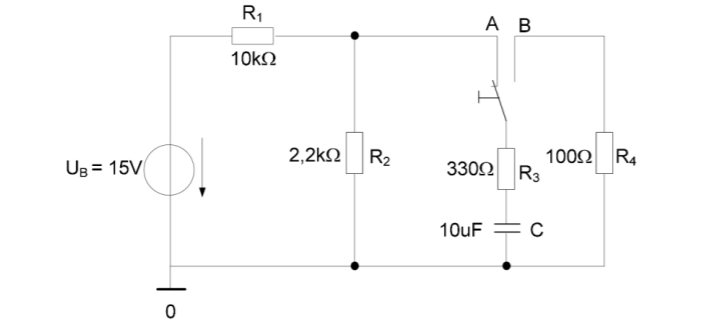
\includegraphics{../assets/images/ET2P4/Schaltplan3.PNG}
        \caption{Schaltplan der dritten Aufgabe mit jeweils zwei Schalterstellungen}
    \end{center}
\end{figure}

\begin{devlist}
    T
    \begin{itemize}
        \item Oszilloskop
        \item Funktionsgenerator
    \end{itemize}
\end{devlist}
\subsection{Aufladung, Schalterstellung A}
Berechnung der Aufladezeitkonsante und der Kondensatorspannung im aufgeladenen Zustand:
\begin{align*}
    \tau_A &= R\cdot C = (330\Omega + \left(\frac{1}{10k\Omega}+\frac{1}{2,2k\Omega}\right)^{-1}) \cdot 10\mu F\\
    \tau_A &= 21,3ms\\\\
    U_c &= U_{R2} = U_B \cdot \left(\frac{R2}{R1+R2}\right) = 15V \cdot \left(\frac{2,2k\Omega}{10k\Omega+2,2k\Omega}\right)\\
    U_c &= 2,7V
\end{align*}
Für den Aufladevorgang lautet die Funktion u$_c$(t) lautet dann:
\begin{align*}
    u_c(t)&= U_0 \cdot (1 - e^{-\frac{t}{RC}})\\
    u_c(t)&= 2,7V \cdot (1 - e^{-\frac{t}{21,3ms}})
\end{align*}
Skizze:
\subsubsection{Messung mit Oszilloskop}
 
\subsection{Entladung, Schalterstellung B}
Berechnung der Entladezeitkonstante $\tau_E$:
\begin{align*}
    \tau_E &= R\cdot C = (330\Omega + 100\Omega) \cdot 10\mu F \\
    \tau_E &= 430\mu s
\end{align*}
Die dazugehörige Entladefunktion u$_c$(t) lautet:
\begin{align*}
    u_c(t)&= U_0 \cdot e^{-\frac{t}{RC}}\\
    u_c(t)&= 2,7V \cdot e^{-\frac{t}{470\mu s}}
\end{align*}
\subsubsection{Messung mit Oszilloskop}
\subsection{Vergleich der gemessenen Zeitkonstanten $\tau_A$ und $\tau_E$}

\end{document}